\section{Experimento BRDF Ashikhmin-Shirley}\label{sec:ashikhmin-shirley}

Neste experimento utilizamos uma BRDF anisotrópica desenvolvida por Ashikhmin-Shirley \cite{ashikhmin2000anisotropic}, que apresenta um modelo de reflexão não uniforme. A descrição matemática está presente na \autoref{fig-ashikhmin-shirley-close-to-original-eqlang-latex}, com o código fonte em \texttt{EquationLang} disponível no \autoref{cod-ashikhmin-shirley-close-to-original-eqlang-pt-1} e \autoref{cod-ashikhmin-shirley-close-to-original-eqlang-pt-2}. Os códigos gerados em GLSL são apresentados nos \autoref{cod-ashikhmin-shirley-close-to-original-glsl-pt-1} e \autoref{cod-ashikhmin-shirley-close-to-original-glsl-pt-2}. A renderização dos objetos 3D pode ser observada na \autoref{fig-ashikhmin-shirley-close-to-original-eqlang} e os plots correspondentes estão na \autoref{fig-ashikhmin-shirley-close-to-original-plots}.

%%%%%%%%%%%%%%%%%%%%%%%%%%%%%%%%%%%%%%%%%%%%%%%%%
\subsection{Representação em documento \LaTeX{}}
%%%%%%%%%%%%%%%%%%%%%%%%%%%%%%%%%%%%%%%%%%%%%%%%%
\begin{figure}[H]
    \caption{\label{fig-ashikhmin-shirley-close-to-original-eqlang-latex} \small Equações da BRDF do experimento ashikhmin-shirley-close-to-original-Kay em documento \LaTeX{}.}
    \begin{center}
        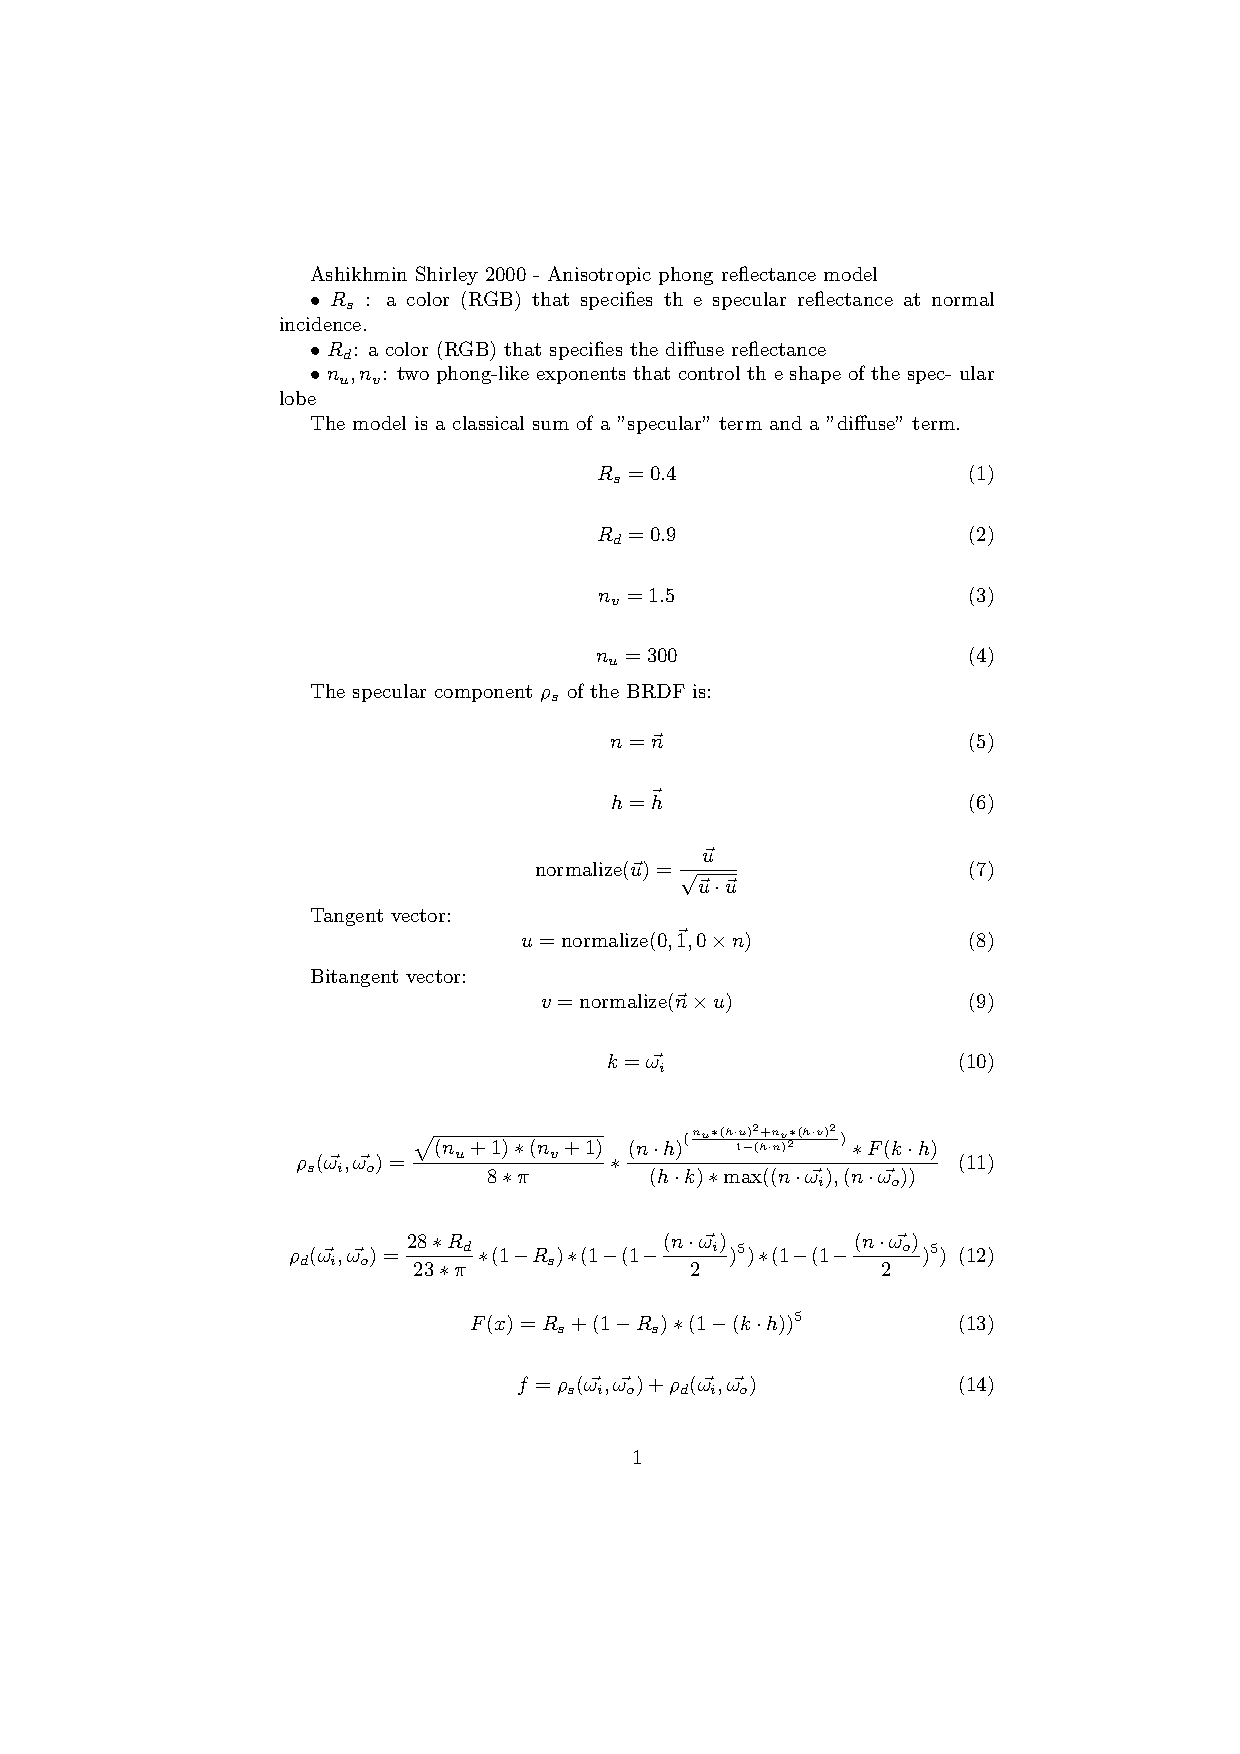
\includegraphics[scale=0.92]{./Imagens/brdfs/ashikhmin-shirley-close-to-original.pdf}
    \end{center}
\end{figure}

%%%%%%%%%%%%%%%%%%%%%%%%%%%%%%%%%%%%%%%%%%%%%%%%%
\subsection{Visualização do Resultado}
%%%%%%%%%%%%%%%%%%%%%%%%%%%%%%%%%%%%%%%%%%%%%%%%%

\begin{figure}[H]
    \caption{\small{Distribuição de Reflexão Especular e Difusa da BRDF}}\label{fig-ashikhmin-shirley-close-to-original-plots}
\minipage{0.48\textwidth}
    \vspace{42px}
  
\includegraphics[width=\linewidth]{./Imagens/brdfs/ashikhmin-shirley-close-to-original-3D-plot}
    % \vspce{0.1px}
    \legend{ \small (a) 3D \textit{plot}}
\endminipage\hfill
\minipage{0.48\textwidth}
  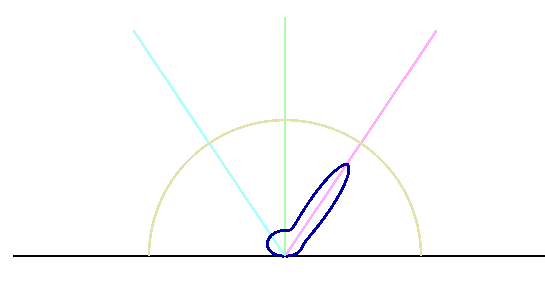
\includegraphics[width=\linewidth]{./Imagens/brdfs/ashikhmin-shirley-close-to-original-polar-plot.png}
    \legend{ \small (b) \textit{Polar plot}}
\endminipage\hfill
\end{figure}

\begin{figure}[H]
    \caption{\small{Objetos 3D renderizados por este experimento}}\label{fig-ashikhmin-shirley-close-to-original-eqlang}
\minipage{0.32\textwidth}
  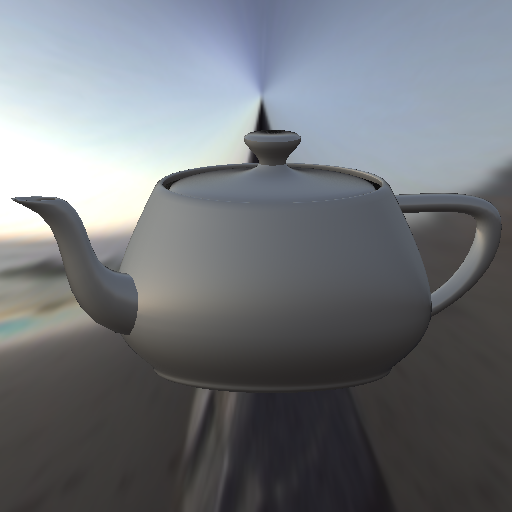
\includegraphics[width=\linewidth]{./Imagens/brdfs/ashikhmin-shirley-close-to-original-teapot.png}
    \legend{ \small (a) \textit{Teapot}}
\endminipage\hfill
\minipage{0.32\textwidth}
  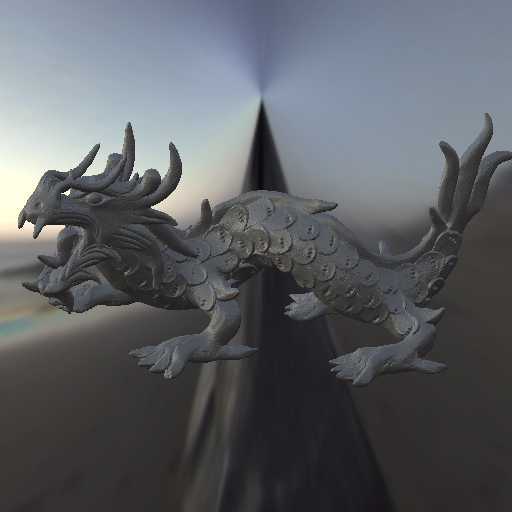
\includegraphics[width=\linewidth]{./Imagens/brdfs/ashikhmin-shirley-close-to-original-dragon.png}
    \legend{ \small (b) Dragão de Stanford}
\endminipage\hfill
\minipage{0.32\textwidth}%
  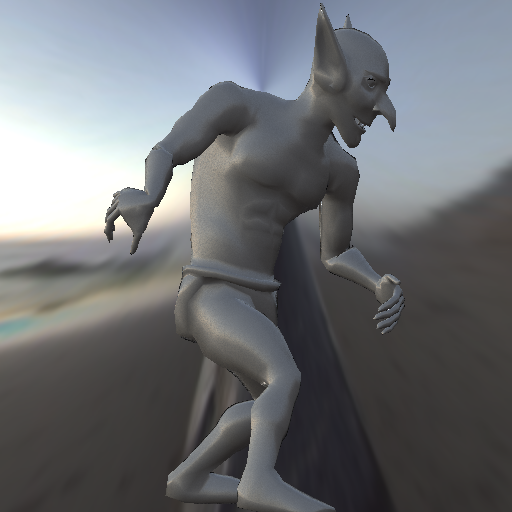
\includegraphics[width=\linewidth]{./Imagens/brdfs/ashikhmin-shirley-close-to-original-goblin.png}
    \legend{ \small (c) Goblin}
\endminipage
\end{figure}

%%%%%%%%%%%%%%%%%%%%%%%%%%%%%%%%%%%%%%%%%%%%%%%%%
\subsection{Código GLSL Gerado}
%%%%%%%%%%%%%%%%%%%%%%%%%%%%%%%%%%%%%%%%%%%%%%%%%
\begin{codigo}[H]
    \caption{\small Saida do compilador, código GLSL da BRDF deste experimento (parte 1). }
    \label{cod-ashikhmin-shirley-close-to-original-glsl-pt-1}
\begin{lstlisting}[language=C, inputencoding=utf8]
analytic ::begin parameters
#[type][name][min val][max val][default val]
::end parameters
::begin shader
//////////// START OF BUILTINS DECLARTION ////////////
vec3 var_0_vec_h;
vec3 var_3_vec_n;
float var_10_theta_h;
float var_11_theta_d;
float var_1_pi;
float var_2_epsilon;
vec3 var_4_vec_omega_i;
float var_5_theta_i;
float var_6_phi_i;
vec3 var_7_vec_omega_o;
float var_8_theta_o;
float var_9_phi_o;
//////////// END OF BUILTINS DECLARTION ////////////
//////////// START OF USER DECLARED ////////////
vec3 var_12_k;
float var_13_n_v;
float var_14_n_u;
vec3 var_17_n;
vec3 var_18_u;
vec3 var_19_v;
float var_20_R_s;
vec3 var_21_h;
float var_24_R_d;
float var_27_f;
//////////// END OF USER DECLARED ////////////
//////////// START FUNCTIONS DECLARATIONS ////////////
vec3 var_15_text_normalize(vec3 var_16_vec_u) {
  return (var_16_vec_u / sqrt(dot(var_16_vec_u, var_16_vec_u)));
}
float var_22_F(float var_23_x) {
  return (var_20_R_s + (((1.0 - var_20_R_s)) *
                        pow(((1.0 - (dot(var_12_k, var_21_h)))), 5.0)));
}
float var_25_rho_d(vec3 var_4_vec_omega_i, vec3 var_7_vec_omega_o) {
  return (((((28.0 * var_24_R_d) / (23.0 * var_1_pi)) * ((1.0 - var_20_R_s))) *
       ((1.0 - pow(((1.0 - ((dot(var_17_n, var_4_vec_omega_i)) / 2.0))), 5.0)))) *
      ((1.0 - pow(((1.0 - ((dot(var_17_n, var_7_vec_omega_o)) / 2.0))), 5.0))));
}
\end{lstlisting}
\end{codigo}

\begin{codigo}[H]
    \caption{\small Saida do compilador, código GLSL da BRDF deste experimento  (parte 2). }
    \label{cod-ashikhmin-shirley-close-to-original-glsl-pt-2}
\begin{lstlisting}[language=C, inputencoding=utf8]
float var_26_rho_s(vec3 var_4_vec_omega_i, vec3 var_7_vec_omega_o) {
  return ((sqrt((((var_14_n_u + 1.0)) * ((var_13_n_v + 1.0)))) / (8.0 * var_1_pi)) *
      ((pow((dot(var_17_n, var_21_h)),
            ((((var_14_n_u * pow((dot(var_21_h, var_18_u)), 2.0)) +
            (var_13_n_v * pow((dot(var_21_h, var_19_v)), 2.0))) /
            (1.0 - pow((dot(var_21_h, var_17_n)), 2.0))))) *
        var_22_F(dot(var_12_k, var_21_h))) /
       ((dot(var_21_h, var_12_k)) * max((dot(var_17_n, var_4_vec_omega_i)),
                                        (dot(var_17_n, var_7_vec_omega_o))))));
}
//////////// END FUNCTIONS DECLARATIONS ////////////
vec3 BRDF(vec3 L, vec3 V, vec3 N, vec3 X, vec3 Y) {
  //////////// START OF BUILTINS INITIALIZATION ////////////
  var_0_vec_h = normalize(L + V);
  var_3_vec_n = normalize(N);
  var_1_pi = 3.141592653589793;
  var_2_epsilon = 1.192092896e-07;
  var_4_vec_omega_i = L;
  var_5_theta_i = atan(var_4_vec_omega_i.y, var_4_vec_omega_i.x);
  var_6_phi_i = atan(sqrt(var_4_vec_omega_i.y * var_4_vec_omega_i.y +
                          var_4_vec_omega_i.x * var_4_vec_omega_i.x),
                     var_4_vec_omega_i.z);
  var_7_vec_omega_o = V;
  var_8_theta_o = atan(var_7_vec_omega_o.y, var_7_vec_omega_o.x);
  var_9_phi_o = atan(sqrt(var_7_vec_omega_o.y * var_7_vec_omega_o.y +
                          var_7_vec_omega_o.x * var_7_vec_omega_o.x),
                     var_7_vec_omega_o.z);
  var_10_theta_h = acos(dot(var_0_vec_h, N));
  var_11_theta_d = acos(dot(var_0_vec_h, var_4_vec_omega_i));
  //////////// END OF BUILTINS INITIALIZATION ////////////
  var_12_k = var_4_vec_omega_i;
  var_13_n_v = 1.5;
  var_14_n_u = 300.0;
  var_17_n = var_3_vec_n;
  var_18_u = var_15_text_normalize(cross(vec3(0.0, 1.0, 0.0), var_17_n));
  var_19_v = var_15_text_normalize(cross(var_3_vec_n, var_18_u));
  var_20_R_s = 0.4;
  var_21_h = var_0_vec_h;
  var_24_R_d = 0.9;
  var_27_f = (var_26_rho_s(var_4_vec_omega_i, var_7_vec_omega_o) +
              var_25_rho_d(var_4_vec_omega_i, var_7_vec_omega_o));
  return vec3(var_27_f);
}
\end{lstlisting}
\end{codigo}

%%%%%%%%%%%%%%%%%%%%%%%%%%%%%%%%%%%%%%%%%%%%%%%%%
\subsection{Código Fonte em \texttt{EquationLang}}
%%%%%%%%%%%%%%%%%%%%%%%%%%%%%%%%%%%%%%%%%%%%%%%%%
\begin{codigo}[H]
    \caption{\small Código fonte da BRDF deste experimento (parte 1).}
    \label{cod-ashikhmin-shirley-close-to-original-eqlang-pt-1}
\begin{lstlisting}[language=tex, frame=none, inputencoding=utf8]
Ashikhmin Shirley 2000 - Anisotropic phong reflectance model

 $R_s$ : a color (RGB) that specifies th e specular reflectance
at normal incidence.

 $R_d$: a color (RGB) that specifies the diffuse reflectance

 $n_u, n_v$: two phong-like exponents that control th e shape of the spec- ular lobe

The model is a classical sum of a "specular" term and a "diffuse" term.

\begin{equation}
    R_s = 0.4
\end{equation}

\begin{equation}
    R_d = 0.9
\end{equation}

\begin{equation}
    n_v = 1.5
\end{equation}

\begin{equation}
    n_u = 300
\end{equation}

The specular component $\rho_s$ of the BRDF is:

\begin{equation}
    n = \vec n
\end{equation}

\begin{equation}
    h = \vec h
\end{equation}
\end{equation}
\end{lstlisting}
\end{codigo}



\begin{codigo}[H]
    \caption{\small Código fonte da BRDF deste experimento (parte 2).}
    \label{cod-ashikhmin-shirley-close-to-original-eqlang-pt-2}
\begin{lstlisting}[language=tex, frame=none, inputencoding=utf8]
\begin{equation}
  \text{normalize}(\vec{u}) = \frac{\vec{u}}{\sqrt{\vec{u} \cdot \vec{u}}}
\end{equation}
Tangent vector:
\begin{equation}
   u = \text{normalize}(\vec{0,1,0} \times n)
Bitangent vector:
\begin{equation}
   v = \text{normalize}(\vec{n} \times u)
\end{equation}

\begin{equation}
    k = \vec{\omega_i}
\end{equation}

\begin{equation}
    \rho_s(\vec{\omega_i}, \vec{\omega_o}) =
        \frac{\sqrt{(n_u+1)*(n_v+1)}}{8*\pi}
        * \frac{(n \cdot h)^{(\frac{n_u * (h \cdot u )^2 + n_v *(h \cdot v)^2}{1-(h \cdot n)^2})}
        * F(k \cdot h)}{(h \cdot k) * \max((n \cdot \vec{\omega_i}), (n \cdot \vec{\omega_o}) )}
\end{equation}

\begin{equation}
    \rho_d(\vec{\omega_i}, \vec{\omega_o}) = \frac{28*R_d}{23*\pi}
        * (1-R_s)
        * (1-(1-\frac{(n \cdot \vec{\omega_i})}{2})^5)
        * (1-(1-\frac{(n \cdot \vec{\omega_o})}{2})^5)
\end{equation}

\begin{equation}
    F(x) = R_s + (1-R_s)*(1-(k \cdot h))^5
\end{equation}

\begin{equation}
    f = \rho_s(\vec{\omega_i}, \vec{\omega_o}) + \rho_d(\vec{\omega_i}, \vec{\omega_o})
\end{equation}
\end{lstlisting}
\end{codigo}
